\documentclass[border=10pt]{standalone}

\usepackage{tikz}
\usepackage{tikzsymbols}
\usetikzlibrary{calc,patterns,shapes.geometric}

\def\centerarc[#1](#2)(#3:#4:#5){\draw[#1] ($(#2)+({#5*cos(#3)},{#5*sin(#3)})$) arc (#3:#4:#5);}

\begin{document}
	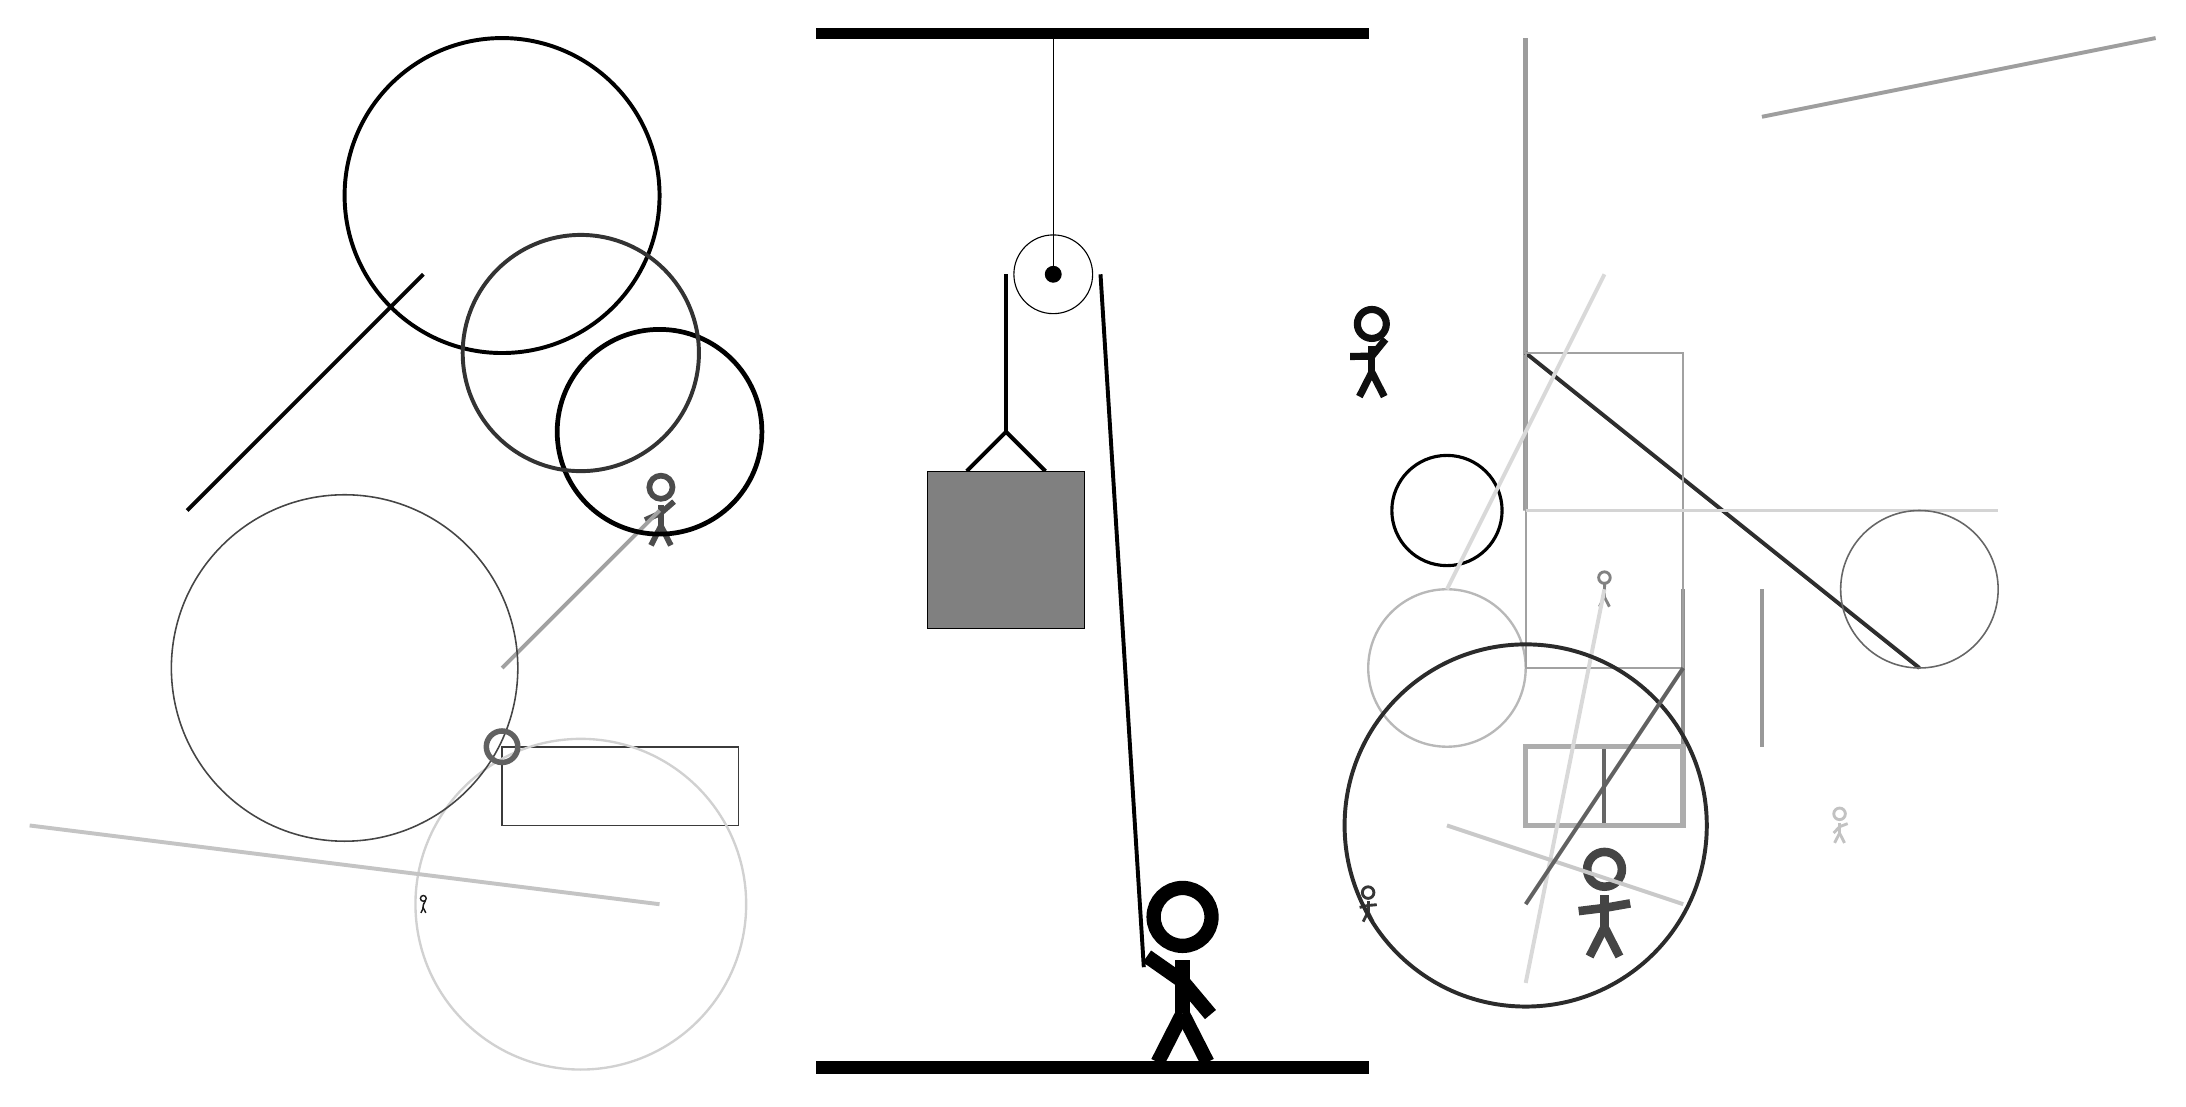
\begin{tikzpicture}
		%%%%% START %%%%%
		
		\draw[fill=black] (-2, 10) rectangle (5, 10.125);
		
		\draw[line width=0.6mm, color=black!39] (7, 10) rectangle (7, 4);
		
		\node[line width=0.4mm, color=black!49] at (8, 3) {\Strichmaxerl[2][80][88]};
		\draw [line width=0.3mm, color=black!28](6, 2) circle (1.0);
		\draw[line width=0.2mm, color=black!77] (-3, 1) rectangle (-6, 0);
		\draw[line width=0.5mm, color=black!60](8, 0) -- (8, 1);
		\draw[line width=0.5mm, color=black!43](9, 3) -- (9, 1);
		\draw [line width=0.3mm, color=black!18](-5, -1) circle (2.1);
		\draw [line width=0.4mm, color=black!100](6, 4) circle (0.7);
		\draw[line width=0.5mm, color=black!82](7, 6) -- (12, 2);
		\node[line width=0.6mm, color=black!70] at (-4, 4) {\Strichmaxerl[4][24][41]};
		\node[line width=0.2mm, color=black!79] at (5, -1) {\Strichmaxerl[2][13][5]};
		\draw[line width=0.5mm, color=black!23](-4, -1) -- (-12, 0);
		\draw[line width=0.7mm, color=black!32] (7, 0) rectangle (9, 1);
		
		\node[line width=0.2mm, color=black!73] at (8, -1) {\Strichmaxerl[6][7][10]};
		\draw[line width=0.5mm, color=black!37](-4, 4) -- (-6, 2);
		\draw [line width=0.6mm, color=black!100](-4, 5) circle (1.3);
		\draw[line width=0.2mm, color=black!37] (7, 2) rectangle (9, 6);
		
		\draw[line width=0.5mm, color=black!38](10, 9) -- (15, 10);
		\draw[line width=0.5mm, color=black!15](8, 3) -- (7, -2);
		\node[line width=0.7mm, color=black!89] at (-7, -1) {\Strichmaxerl[1][82][63]};
		\draw[line width=0.5mm, color=black!15](6, 3) -- (8, 7);
		
		\draw[line width=0.5mm, color=black!21](9, -1) -- (6, 0);
		\draw[line width=0.5mm, color=black!17](7, 4) -- (13, 4);
		\draw [line width=0.5mm, color=black!83](7, 0) circle (2.3);
		\draw[line width=0.5mm, color=black!62](9, 2) -- (7, -1);
		\draw [line width=0.5mm, color=black!100](-6, 8) circle (2.0);
		\draw[line width=0.5mm, color=black!40](10, 1) -- (10, 3);
		\draw [line width=0.5mm, color=black!80](-5, 6) circle (1.5);
		\draw [line width=0.2mm, color=black!73](-8, 2) circle (2.2);
		
		\draw[line width=0.5mm, color=black!98](-7, 7) -- (-10, 4);
		\node[line width=0.6mm, color=black!94] at (5, 6) {\Strichmaxerl[5][1][51]};
		
		\draw [line width=0.7mm, color=black!62](-6, 1) circle (0.2);
		\node[line width=0.5mm, color=black!24] at (11, 0) {\Strichmaxerl[2][47][21]};
		\draw [line width=0.2mm, color=black!60](12, 3) circle (1.0);
		
		\draw (1, 7) circle (0.5);
		\draw[fill=black] (1, 7) circle (0.1);
		\draw (1, 10) -- (1, 7);
		
		\draw[line width=0.5mm] (-0.1, 4.5) -- (0.4, 5.0) -- (0.9, 4.5);
		\draw[fill=black!50] (-0.6, 4.5) rectangle (1.4, 2.5);
		
		\draw[line width=0.5mm] (0.4, 7) -- (0.4, 5.0);
		\centerarc[line width=0.5mm](1, 7)(0:180:0.6);
		\draw[line width=0.5mm](1.6, 7) -- (2.15, -1.8);
		
		\node at (2.6, -1.9) {\Strichmaxerl[10][-35][-50]};
		
		\draw[fill=black] (-2, -3) rectangle (5, -3.15);
		
		%%%%% END %%%%%
	\end{tikzpicture}
\end{document}